\documentclass[a4paper, 12pt]{report}
\usepackage[top=2.5cm,bottom=2.5cm,left=2.5cm,right=2.5cm]{geometry}
%-----------------------------------------------------------------------  01
\usepackage[pdftex]{graphicx}
\usepackage{graphics}
%\usepackage{fancyhdr} 
%----------------------------------------------------------------------   02
\usepackage[utf8]{inputenc} 
\usepackage[T1]{fontenc}
\usepackage[french]{babel}
\usepackage{hyperref}
\hypersetup{
	colorlinks,
	citecolor=blue,
	filecolor=blue,
	linkcolor=blue,
	urlcolor=blue
}
\usepackage{array}
\usepackage{tabularx}
\usepackage{titlesec}

\usepackage{makecell, amssymb, amsthm, mathtools, rotating, colortbl, enumitem, nomencl, latexsym, bookmark, url, subcaption, float, multirow, algorithm, algorithmic, color}
\usepackage{arabtex, utf8}
%\setcode{utf8}
\usepackage[nomain, acronym]{glossaries}




%-----------------------------------------------------------------------   03
\linespread{1.5}

%%%%%%%%%%%%%%%%%%%%%%%%%%%%%%%%%%%%%%%%%%%%%%%%%%%%%%%% fix Subsection Error %%%%%%%%%%%%%
\setcounter{tocdepth}{3}
\setcounter{secnumdepth}{3}
\usepackage{lipsum}

\begin{document} 
	\begin{titlepage}
		%------------------------------------------------------------------------  04
		\begin{figure}[htbp]
			\hbox{
				\hspace*{-1.4cm}
				
\includegraphics[width=100px]{./Template LaTeX/Images/ISCAE.jpg}
				\hspace*{11cm}
				
\includegraphics[width=80px]{./Template LaTeX/Images/logoUniv.jpg}
			}
		\end{figure}
		%-------------------------------------------------------------------------- 05
		\vspace {-4cm}
		
		\begin{center}
			\vspace{1cm}
			
			{\bf République Islamique de Mauritanie } \vspace{-0.2cm}\\
			{\bf	Ministre de l’Enseignement Supérieur et de la } \vspace{-0.2cm}\\
			
			{\bf Recherche Scientifique }\\
			
			\vspace{2cm}
			
			%------------------------------------------------------------------------- 06
			\bf{MÉMOIRE DE STAGE DE FIN D'ÉTUDES} \\
			\vspace{1cm}
			{\bf Présenté en vue de l’obtention du } \vspace{-0.2cm}\\
			{\bf Diplôme de Master Professionnel en Informatique}\vspace{-0.2cm}\\
				{\bf	Appliquée à la Gestion (MPIAG)}\\ \vspace{0.2cm}
				{\bf Par :}\\ \vspace{0.2cm}
					{\bf Mohamed Lemine Salem M’bedah (IE18689) }\\ \vspace{0.2cm}
			\huge{\textbf{Thème}}\\ 
			\noindent\rule{\textwidth}{1mm}
			\Large{\bf{CREATION D’UN SYSTEME DE GESTION DE RELATION CLIENT (CRM)  ET DE KYC  \\ (KNOW YOUR CUSTOMER)}}
			\noindent\rule{\textwidth}{1mm}
		\end{center}
		\vspace{0cm}
		%-------------------------------------------------------------------------- 07
		\begin{center}
			
			{\bf Encadré par :}\\
			{Dr. Cheikh Dhib} \\
			{Mr. Mboirick Mohamed} \\
			{\bf Réalisé au sein de CADORIM }
			
			
		\end{center}
		\begin{figure}[htbp]
		\hbox{
			\hspace*{5cm}
			
\includegraphics[width=150px]{./Template LaTeX/Images/cado_logo.png}
		}
		\end{figure}
		
		\begin{center}
			Année universitaire 2021-2022
		\end{center}
		%--------------------------------------------------------------------------- 08
	\end{titlepage}
		\chapter*{DEDICACES} \label{chap:1Dedicaces}
		%\addcontentsline{toc}{chapter}{DEDICACES} 
		Les mots ne sauront traduire ce qui est dans le cœur, mais je vais rassembler mon vocabulaire et dire : je dédie cet humble travail à mes chers parents pour leur soutien tout au long de mon parcours universitaire, qui ont été les encouragements dans les moments de détresse, l'exhortation en période de prospérité, le soutien lors de la chute et le guide lors de la montée,qui n’a pas hésité un instant à m’aider jusqu’à ce que je suis arrivé là où
		je suis maintenant. Tous les remerciements et gratitudes ne remplissent pas leur droit.
		%sa signification
			%\textbf{<< Dis, mon Seigneur, aie pitié d'eux comme ils m'ont élevé quand j'étais jeune >>}
		\thispagestyle{empty} 
		\chapter*{REMERCIEMENTS} \label{chap:1REMERCIEMENTS}
		%\addcontentsline{toc}{chapter}{REMERCIEMENTS} 
		\textit{
			Ce n’est pas parce que la tradition l’exige que cette page se trouve dans ce rapport;
			mais par ce que les gens à qui s’adressent mes remerciements les méritent vraiment.
			\newline
			J’adresse mes remerciements les plus chaleureux envers : 
			\begin{enumerate}
				 \item[•] \textbf{Dr. Cheikh Dhib,} l'ancien coordinateur de MPIAG, ainsi que \textbf{Dr. Emani Mohamed Sidi} le nouveau coordinateur et l’ensemble du corps
				 professoral et administratif de l’ISCAE.
				 Et pour avoir suivi et dirigé l’évolution de mon travail, ainsi que les encouragements, conseils et orientations réguliers qu’il m’a prodigués.
				 Je vous suis infiniment reconnaissant pour votre grande disponibilité et l’intérêt que vous avez porté à ce travail;
				  \item[•] \textbf{Mr. Mboirick Mohamed, } responsable technique et mon maître de stage, pour ça
				  disponibilité, sa gentillesse, son attention particulière à l’égard de ce travail. Et pour
				  avoir mis les moyens nécessaires au bon déroulement de ce stage de six mois et à
				  la réalisation de ce travail ; Je vous suis infiniment reconnaissant pour votre grande
				  disponibilité et l’intérêt que vous avez porté à ce travail ;
			\end{enumerate}
			Toutes les personnes qui de près ou de loin, ont contribué à la réalisation de ce travail.
		 }
	 \thispagestyle{empty}
	 \chapter*{AVANT-PROPOS} \label{chap:1AVANT-PROPOS}
	%\addcontentsline{toc}{chapter}{AVANT-PROPOS}
	L’Institut Supérieur de Comptabilité et d’Administration des Entreprises est un établissement public d’enseignement supérieur et de recherche, placé sous la tutelle du Ministère en charge de l’Enseignement Supérieur, crée en 2009, par décret N° 2009-161 du 29 avril 2009.
	\newline
	L’ISCAE compte deux (2) départements et dans le cadre de leur formation, les étudiants qui sont en fin de cycle sont tenus d’effectuer un stage pratique au sein d’une entreprise ou d’un service informatique.
	\thispagestyle{empty}
	\chapter*{RESUME} \label{chap:1Resumé}
	Dans le cadre de l’obtention de notre diplôme de MASTER en Système d’information
	à Institut Supérieur de comptabilité et d’administration des entreprises nous avons été
	appelés à réaliser un projet de fin d’études afin de clôturer notre formation du second cycle
	universitaire. C’est ainsi qu’on a eu l’occasion d’enrichir davantage nos connaissances
	théoriques par la création d’un système de gestion de relation client (CRM) et de kyc
	 (KNOW YOUR CUSTOMER). Ce sujet a été proposé par la start-up Cadorim qui exerce
	 Dans le domaine du transfert d’argent de l’Europe vers la Mauritanie. Pour atteindre cet
	 Objectifs, nous avons utilisé les infrastructures technologiques suivantes : *UML : pour la
	 modélisation des données *Framework Flutter : pour le front-end (Interface utilisateur).
	 *Framework Laravel : pour le back-end (Interface Administrateur).
	Le système de gestion de base de données (SGBD) est MySQL.
	Il faut noter que pour modéliser et gérer les différents diagrammes UML l'outil
	StarUML nous a été utile.
	
	\thispagestyle{empty}
	\chapter*{LISTE DES ABRÉVIATIONS} \label{chap:1SIGLES ET ABREVIATIONS}
	%\addcontentsline{toc}{chapter}{SIGLES ET ABREVIATIONS}
	Je présente ici certains sigles et abréviations que nous utiliserons dans le document.
	\newline\newline
	\textbf{ISCAE} : Institut Supérieur de Comptabilité et d’Administration des Entreprises \newline
	\textbf{MPIAG} : Master Professionnel en Informatique Appliquée à la Gestion \newline
	\textbf{API} : Application Programming Interface \newline
	\textbf{MVC} : Modèle Vue Contrôleur \newline
	\textbf{HTTP} : Hypertext Transfer Protocol \newline
	\textbf{HTTPS} : HyperText Transfer Protocol Secure \newline
	\textbf{UML} : Unified Modeling Language \newline
	\textbf{SQL} : Structured Query Language \newline
	\textbf{JSON} : JavaScript Object Notation \newline
	\textbf{XP} : eXtreme Programming \newline
	\textbf{IIS} : Internet Information Services \newline
	\textbf{DAO} : Data Access Object \newline
	\textbf{AAB} : Android App Bundles \newline
	\textbf{APK} : Android Package Kit \newline
	\textbf{IDE} : Integrated Development Environment (Environnement de Développement Intégré) \newline
	\textbf{MERISE} : Méthode d’Étude et de Réalisation Informatique par les Sous-Ensembles ou pour les Systèmes d’Entreprise \newline
	\textbf{OPT} : One-Time Password \newline
	\textbf{SGBD} : Système de Gestion de Bases de Données \newline
	\textbf{SGBDR} : Système de Gestion de Bases de Données Relationnelle \newline
	\textbf{SOA} : Service Oriented Architecture \newline
	\textbf{OCR} : Optical Character Recognition  \newline
	\textbf{MRZ} : Machine-Readable Zone  
	\thispagestyle{empty}
	
	\tableofcontents
	\thispagestyle{empty}
	\let\cleardoublepage\clearpage

\chapter{Introduction générale}
\label{sec:DescriptionDuProjet}

Savoir qui est votre client et adopter des protocoles pour prévenir la criminalité financière sont des défis permanents pour les institutions financières. De manière significative, les institutions financières (y compris les banques, les coopératives de crédit et les sociétés financières du Fortune 50) doivent se conformer à un ensemble de réglementations de plus en plus complexes pour la vérification de l'identité des clients appelée KYC.

KYC, également connu sous le nom de "Know Your Customer" ou "Know Your Client", est un ensemble de procédures permettant de vérifier l'identité d'un client avant ou pendant les transactions avec les banques et autres institutions financières. Le respect des réglementations KYC peut aider à tenir à distance le blanchiment d'argent, le financement du terrorisme et d'autres stratagèmes de fraude courants. En vérifiant d'abord l'identité et les intentions d'un client au moment de l'ouverture du compte, puis en comprenant ses habitudes de transaction, les institutions financières sont en mesure d'identifier plus précisément les activités suspectes. 

Les institutions financières sont soumises à des normes de plus en plus strictes en matière de lois KYC. Ils doivent dépenser plus d'argent pour se conformer à KYC ou être passibles de lourdes amendes. Ces réglementations signifient que presque toutes les entreprises, plateformes ou organisations qui interagissent avec une institution financière pour ouvrir un compte ou effectuer des transactions devront se conformer à ces obligations.

La gestion de la relation client (CRM) est la combinaison de pratiques, de stratégies et de technologies que les entreprises utilisent pour gérer et analyser les interactions et les données client tout au long du cycle de vie du client. L'objectif est d'améliorer les relations de service client, de contribuer à la fidélisation de la clientèle et de stimuler la croissance des ventes. Les systèmes CRM compilent les données client à travers différents canaux, ou points de contact, entre le client et l'entreprise, qui peuvent inclure le site Web de l'entreprise, le téléphone, le chat en direct, le publipostage, les supports marketing et les réseaux sociaux. Les systèmes CRM peuvent également donner aux membres du personnel en contact avec les clients des informations détaillées sur les informations personnelles des clients, l'historique des achats, les préférences et les préoccupations d'achat.


\section{Motivations}

KYC est un moyen de rendre la vérification de l'identité des clients plus précise et moins vulnérable à la fraude.

KYC doivent être effectuées lors de l'intégration d'un nouveau client, mais il est préférable de répéter ces vérifications de temps en temps, pour s'assurer que tout est comme il se doit. En surveillant les comptes clients de cette manière, les comportements suspects peuvent être signalés plus rapidement.

Un système CRM fournit des flux de travail automatisés qui permettent à votre équipe marketing de consacrer plus de temps à des tâches stratégiques, telles que la création de campagnes marketing qui résonnent, l'analyse des données de ces campagnes et le test de différentes approches basées sur ces analyses. Les agents du service client peuvent passer leur temps à travailler avec des clients qui ont des questions, des problèmes ou des besoins plus complexes. En bref, avec des processus de service client plus efficaces, les entreprises peuvent établir de meilleures relations avec leurs clients.

\section{Problématiques}

En réalité, la réalisation d'une application,qui applique le principe de KYC et integre un  système CRM,
nécessite
de faire face à des problématiques diverses et complexes. Ainsi, la société a décidé de se contenter,
dans un premier temps, Mise en place d’un système d’extration des donnees à partir des images et traitement des ces donnees(carte d'identité ou passeport).
Ce sujet soulève de nombreuses questions aux implications différentes. Comment peut extraire le texte apartir de l'image? Comment sera-t-il traité ? Comment peut-il être utilisé dans le principe KYC ? Comment pouvons-nous obtenir un système CRM intégré ?


\section{Objectifs}

La mise en place d'une application pour appliquer l'ide de KYC en basant sur les différent technologie disponible . En basan sur l'extraction du text apartir d'une imange OCR on peut extracter la code MRZ apartir d'une imange du piece d'idendite ou passport est passe le code a un algorithem qui permer de d'etecter les information personnel.



	\chapter{Contexte général du projet}
%\chapter{Présentation de l’entreprise}
\label{chap:introduction}
\section{Présentation du lieu de stage}
%\pagenumbering{arabic}
\subsection{Introduction}
\begin{figure}[h]
	
\includegraphics[scale=0.14]{./Template LaTeX/Images/cado_logo.png}
	\centering
	\caption{CADOROM}
\end{figure}
CADORIM est une société de transfert d’argent mauritanienne basée à Nouakchott,
fondée fin 2018 par un entrepreneur mauritanien, titulaire d'un doctorat en
mathématiques,
CADORIM consiste a transférer de l’argent depuis n’importe quel pays dans le
monde vers ses proches en Mauritanie. Notre objectif et de fourni une plateforme
numérique permet à l’utilisateur de régler ses commandes en toute sécurité et
confidentialité assurée par le service de PayPal qui est mondialement connu pour sa
fiabilité et simplicité.t Pour effectuer un paiement il suffit d'une simple carte bancaire
ou un compte PayPal . et une éventuelle possibilité de virement bancaire.
CADORIM a été élu comme le champion de Banque Centrale de Mauritanie (BCM )
1ère édition 2019 Fintech Challenge,
Le siège social de CADORIM est situé à marche capital , Nouakchott, Mauritanie,
immatriculée au registre du commerce.
\subsection{Missions}
CADORIM offre une large palette de prestations organisées autour des activités suivantes :
\begin{enumerate}
	
	\item Maintenance et amélioration de leurs propres applications (CadoRim et MauriPay)
	\item Développement des applications 
	\item Des agences des reçoivent d'argent et de service client
	
\end{enumerate}
\subsection{Organigramme}
La structure organisationnelle de CADORIM comprend :
\begin{figure}[h]
	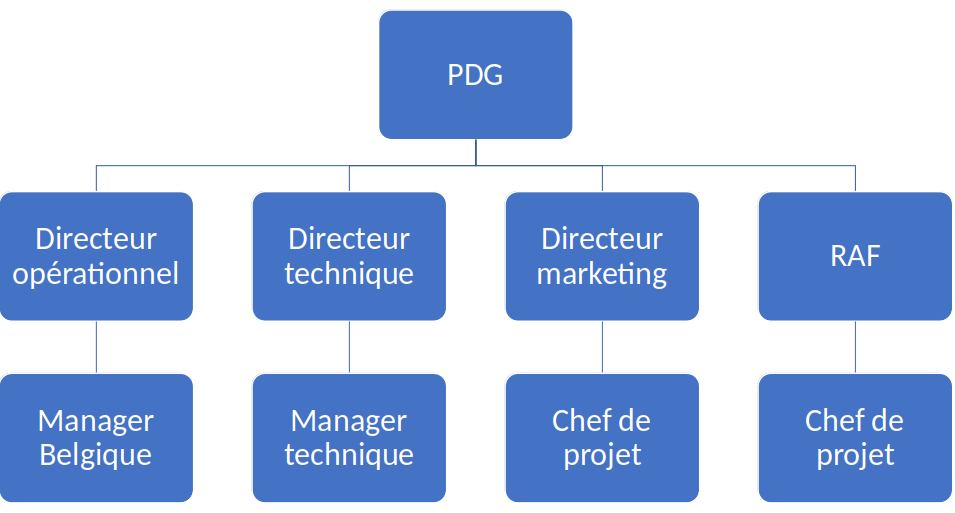
\includegraphics[scale=0.8,width=400px]{./Template LaTeX/Images/og.png}
	\centering
	\caption{Organigramme du CADORIM}
\end{figure}
\begin{comment}
	content...

\subsection{Planification du projet}
J'effectuais le diagramme de Gantt, pour avoir une meilleure compréhension de la chronologie des étapes de mon projet.
\newline
\newline
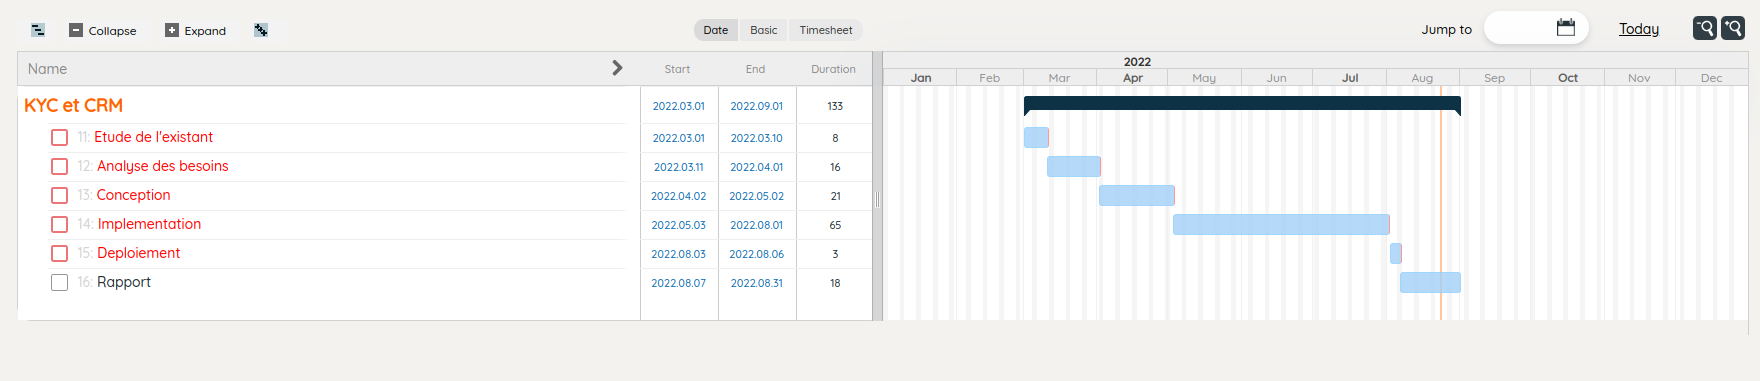
\includegraphics[width=500px,height=175px]{./Template LaTeX/Images/gantt.png}
\newline
Le projet est subdivisé en plusieurs phases.
\begin{enumerate}
\item Une phase comprenant l’étude de l’existant et analyse des besoins, en
intervenant les différents acteurs du projet.
\item Une phase de conception consistant à modéliser et formaliser les
données brutes du cahier de charge
\item Une phase d’implémentation consiste à traduire techniquement les
données provenant de la conception.
\item Déploiement : externalisation des ressources.
\end{enumerate}
\end{comment}
\newpage
\section{Description du projet}
%%%%%%%%%%%%%%%%%%%%%%%%%%%%%%%%%%%%% New add from Introduction %%%%%%%%%%%%%%%%%%%%%
\begin{comment}
	content...

Savoir qui est votre client et adopter des protocoles pour prévenir la criminalité financière sont des défis permanents pour les institutions financières. De manière significative, les institutions financières (y compris les banques, les coopératives de crédit et les sociétés financières du Fortune 50) doivent se conformer à un ensemble des réglementations de plus en plus complexes pour la vérification de l'identité des clients appelée KYC.

KYC, également connu sous le nom de "Know Your Customer" ou "Know Your Client", est un ensemble de procédures permettant de vérifier l'identité d'un client avant ou pendant les transactions avec les banques et autres institutions financières. Le respect des réglementations KYC peut aider à tenir à distance le blanchiment d'argent, le financement du terrorisme et d'autres stratagèmes de fraude courants. En vérifiant d'abord l'identité et les intentions d'un client au moment de l'ouverture du compte, puis en comprenant ses habitudes de transaction, les institutions financières sont en mesure d'identifier plus précisément les activités suspectes. 

Les institutions financières sont soumises à des normes de plus en plus strictes en matière de lois KYC. Ils doivent dépenser plus d'argent pour se conformer à KYC ou être passibles de lourdes amendes. Ces réglementations signifient que presque toutes les entreprises, plateformes ou organisations qui interagissent avec une institution financière pour ouvrir un compte ou effectuer des transactions devront se conformer à ces obligations.

La gestion de la relation client (CRM) est la combinaison de pratiques, de stratégies et de technologies que les entreprises utilisent pour gérer et analyser les interactions et les données client tout au long du cycle de vie du client. L'objectif est d'améliorer les relations de service client, de contribuer à la fidélisation de la clientèle et de stimuler la croissance des ventes. Les systèmes CRM compilent les données client à travers différents canaux, ou points de contact, entre le client et l'entreprise, qui peuvent inclure le site Web de l'entreprise, le téléphone, le chat en direct, le publipostage, les supports marketing et les réseaux sociaux. Les systèmes CRM peuvent également donner aux membres du personnel en contact avec les clients des informations détaillées sur les informations personnelles des clients, l'historique des achats, les préférences et les préoccupations d'achat.


\subsection{Motivations}    

KYC est un moyen de rendre la vérification de l'identité des clients plus précise et moins vulnérable à la fraude.

KYC doivent être effectuées lors de l'intégration d'un nouveau client, mais il est préférable de répéter ces vérifications de temps en temps, pour s'assurer que tout est comme il se doit. En surveillant les comptes clients de cette manière, les comportements suspects peuvent être signalés plus rapidement.

Un système CRM fournit des flux de travail automatisés qui permettent à votre équipe marketing de consacrer plus de temps à des tâches stratégiques, telles que la création de campagnes marketing qui résonnent, l'analyse des données de ces campagnes et le test de différentes approches basées sur ces analyses. Les agents du service client peuvent passer leur temps à travailler avec des clients qui ont des questions, des problèmes ou des besoins plus complexes. En bref, avec des processus de service client plus efficaces, les entreprises peuvent établir de meilleures relations avec leurs clients.
\end{comment}
\subsection{Problématiques}	

En réalité, la réalisation d'une application,qui applique le principe de KYC et integre un  système CRM,
nécessite
de faire face à des problématiques diverses et complexes. Ainsi, la société a décidé de se contenter,
dans un premier temps, Mise en place d’un système d’extration des donnees à partir des images (carte d'identité ou passeport) et traitement des ces donnees.
Ce sujet soulève de nombreuses questions aux implications différentes. Comment peut extraire le texte apartir de l'image? Comment sera-t-il traité ? Comment peut-il être utilisé dans le principe KYC ? Comment pouvons-nous obtenir un système CRM intégré ?


\subsection{Objectifs}

La mise en place d'une application pour appliquer l'ide de KYC en basant sur les différent technologie disponible . En basan sur l'extraction du text apartir d'une imange OCR on peut extracter la code MRZ apartir d'une imange du piece d'idendite ou passport est passe le code a un algorithem qui permer de d'etecter les information personnel.





	%\chapter{Conception du projet}
%\label{sec:EnvironnementDeTravail}
\chapter{Analyse fonctionnelle et conceptuelle}
\label{sec:Analyse fonctionnelle et conceptuelle}
%Durant la réalisation de ce projet, nous avons essayé d’utiliser différents
%outils de développement, d’une part afin de rendre la tâche de la
%réalisation plus facile, d’autre part pour que notre système soit robuste et
%répond parfaitement a nos besoins , et que nos interfaces soient claires et
%faciles à utiliser.

%\section{Choix de langage de modélisation :}
\section{Analyse fonctionnelle}
%Dans cette section, je présente le langage et le logiciel de modélisation que j’ai utilisé pour concevoir notre solution.
\begin{comment}
	content...

\subsection{UML}
On a utilisé UML comme langage de modélisation.
Langage de modélisation unifié UML (Unified modeling Langage) un
consiste a modéliser une application logicielle d'une façon standard
dans le cadre de conception orientée objet.
UML consiste a couvrir le cycle de vie d'un logiciel depuis la
spécification des besoins jusqu'au codage en offrant plusieurs
moyens de description et de modélisation des acteurs.
\section{Choix de logiciel de modélisation :}
\subsection{Visual Paradigm  en ligne} 
Visual Paradigm  en ligne est un outil de création de diagrammes en ligne. Vous pouvez créer un nombre illimité de diagrammes, graphiques et autres visuels à partir d’un large éventail de types de diagrammes, y compris UML, organigrammes, BPMN, ERD, DFD, ArchiMate et autres.
%%%%%%%%%%%%%%%%%%%%%%%%%%%%%%%%%%%%%%%%%%%%%%%%%%%%%%%%% Tests %%%%%%%%%%%%%%%%%%%%%%%%%%
\section{Diagramme UML}
\begin{comment}
\begin{table}
		
	\caption{Rôles des diagrammes UML utilisés.}
	\label{table:kysymys}
\begin{tabular}{|c|p{11cm}|}
	
	\hline
	\large \bfseries Diagramme & \large \bfseries Rôle\\
	\hline
	Diagramme de cas d’utilisation & Il consiste à donner une vision globale sur les principales fonctionnalités
	(chaque fonctionnalité représente un cas d’utilisateur) d’une application .  \\
	\hline
	Diagramme d’activité &  Fournir une vue du comportement d'un système en décrivant la séquence d'actions d'un processus.    \\
	\hline
	Diagramme de séquence &Permettent d'identifier les classes requises par un système et le comportement des objets de classes au cours des interactions.  \\
	\hline
	Diagramme de classe    &Le diagramme de classes représente généralement un schéma utilisé en génie
	logiciel pour modéliser un problème bien précis, sous forme des classes et des
	interfaces ainsi que les différentes relations entre celles-ci. \\
	\hline
	
\end{tabular}

\end{table}
\end{comment}
%Table \ref{table:kysymys} on page \pageref{table:kysymys} refers to the ...

\subsection{Diagramme de cas d’utilisation}
\begin{figure}[h!]
	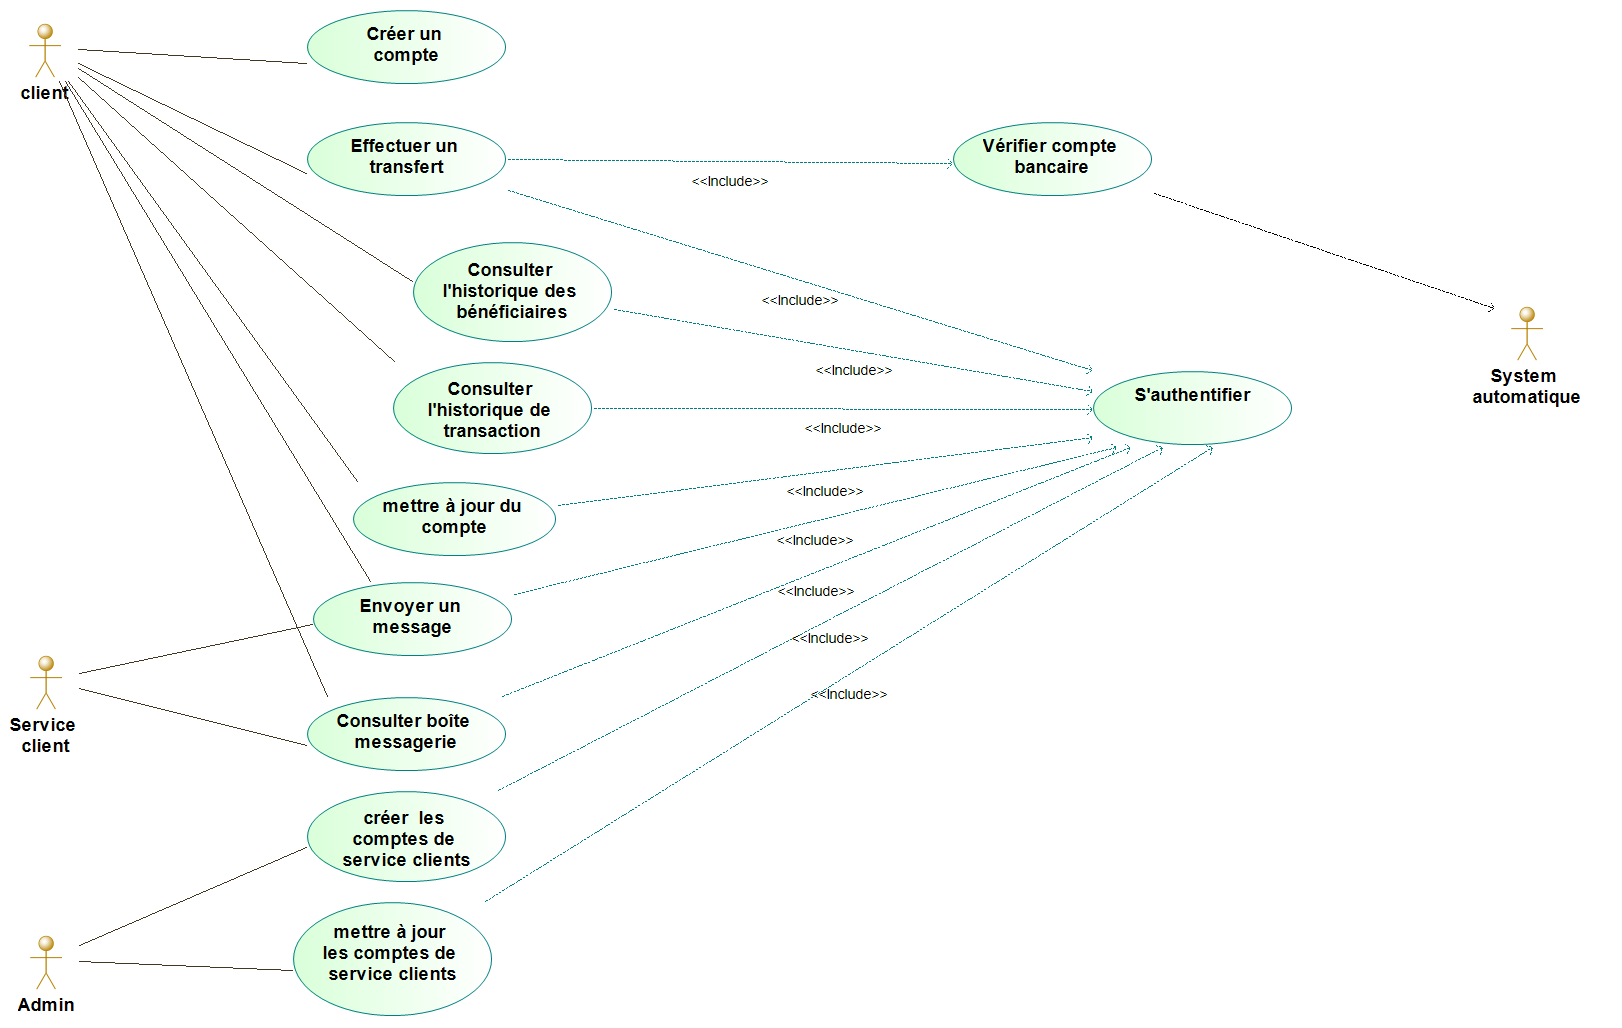
\includegraphics[width=18cm, height=12cm]{./Template LaTeX/Images/use_case.png}
	\caption{Diagramme de cas d’utilisation.}
	\label{fig1:use_case}
\end{figure}
%\textbf{Description détaillée des cas d'utilisation :}
\begin{comment}

\begin{table}[h]
	\begin{tabular}{|m{5cm}|m{2cm}|m{10cm}|}
		\hline
		\textbf{Cas d’utilisation} & \textbf{Acteur} & \textbf{Description}\\
		\hline
		\textbf{Créer un compte }&Client&L'utilisateur se renseigne pour créer un compte au sein de Cadorim pour
		pouvoir accéder au fonctionnalités proposées .\\
		\hline
		\textbf{S’authentifier}&Client&L'utilisateur saisit son identifiant et son mot de passe pour
		accéder aux fonctionnalités.\\
		\hline
		\textbf{Effectuer un transfert}&Client&L'utilisateur saisi le numéro du bénéficiaire et le montant a transférer.
		Une page de vérification avec les informations saisies.
		Transfère le montant vers le bénéficiaire.\\
		\hline
		\textbf{Créer un compte}&Client&L'utilisateur se renseigne pour créer un compte au sein de mauripay pour
		pouvoir accéder au fonctionnalités proposées .\\
		\hline
		\textbf{Créer un compte}&Client&L'utilisateur se renseigne pour créer un compte au sein de mauripay pour
		pouvoir accéder au fonctionnalités proposées .\\
		\hline
		\textbf{Créer un compte}&Client&L'utilisateur se renseigne pour créer un compte au sein de mauripay pour
		pouvoir accéder au fonctionnalités proposées .\\
		\hline
		
	
			
	\end{tabular}
	\caption{Description détaillée des cas d'utilisation}
	\label{4.1}
\end{table}
\end{comment}


	%\textbf{• Description détaillée des cas d'utilisation  :}
\begin{comment}
	
\begin{table}[h]
	\begin{tabular}{|m{4cm}|m{13.5cm}|}
		\hline
		\textbf{Cas d’utilisation}   \textbf{Description}\\
		\hline
		Créer un compte&L'utilisateur se renseigne pour créer un compte au sein de Cadorim pour
		pouvoir accéder au fonctionnalités proposées .\\
		\hline
		S’authentifier&L'utilisateur saisit son identifiant et son mot de passe pour
		accéder aux fonctionnalités.\\
		\hline
		Effectuer un transfert&L'utilisateur saisi le montant a transférer et les informations de  bénéficiaire.
		\newline Une page de vérification avec les informations saisies.
		\newline Transfère le montant vers le bénéficiaire.\\
		\hline
		Consulter l'historique des bénéficaires&L'utilisateur peut voire liste des bénéficaires \\
		\hline
		Consulter l'historique des transactions&L'utilisateur peut voire liste des transactions\\
		\hline
		mettre à jour du compte&L'utilisateur se renseigne pour créer un compte au sein de mauripay pour
		pouvoir accéder au fonctionnalités proposées .\\
		\hline
		Envoyer un message&L'utilisateur se renseigne pour créer un compte au sein de mauripay pour
		pouvoir accéder au fonctionnalités proposées .\\
		\hline
			Consulter boite \newline messagerie&L'utilisateur se renseigne pour créer un compte au sein de mauripay pour
		pouvoir accéder au fonctionnalités proposées .\\
		\hline
		
		
		
	\end{tabular}
	\caption{Description détaillée des cas d'utilisation d'acteur client}
	\label{4.1}
\end{table}
	content...
\end{comment}
%\newpage
\textbf{\hspace*{-1cm}• Description détaillée des cas d'utilisation  :\newline}
\begin{table}[h]
	\hspace*{-2cm}
	\begin{tabular}{|m{19.8cm}|}
		\hline
		\begin{center}
		 \textbf{Cas d’utilisation : Créer un compte, S’authentifier et Créer les comptes de service clients }
		\end{center}
		\\
		[-4ex] 
		\hline
			\begin{tabular}{m{3cm}|m{14cm}}
			
				\centering 	\textbf{Titre} & Créer un compte , S’authentifier , Créer les comptes de service clients
				\\
				[0ex] 
			\end{tabular}
		\\
		
		\hline
			\begin{tabular}{m{3cm}|m{14cm}}
			
			\centering 	\textbf{But} & Créer un compte pour accéder aux fonctionnalités de l’application 	\\
			[0ex] 
			
		\end{tabular}
		\\
		\hline
			\begin{tabular}{m{3cm}|m{15.5cm}}
			
			\centering 	\textbf{Résumé} & L'utilisateur doit remplir un formulaire d’inscription et identifier électroniquement leur document comme des pièces d’identité (carte d’identité, passeport ) à partir de leur caméra du téléphone puis valide son action.\newline Le système effectue une vérification puis une mise à jour de la base de données.
			\\
			[0ex] 
		\end{tabular}
		\\
		
		\hline
			\begin{tabular}{m{3cm}|m{14cm}}
			
			\centering 	\textbf{Acteurs } & Client,Admin \\[0ex]
			
		\end{tabular}
		\\
		 
		\hline
		\begin{center}
			\textbf{Descriptions des enchainements}
		\end{center}
		\\
		[-4ex] 
		\hline	
			\begin{tabular}{m{9.3cm}|m{9.3cm}}
			
			\begin{center}
				\textbf{Pré condition}
			\end{center}
		 		& 
		 	\begin{center}
				\textbf{Post condition}
			\end{center}
			\\[-4ex]
		\end{tabular}
		\\
		
		\hline
			\begin{tabular}{m{9.3cm}|m{9.3cm}}
			L'utilisateur doit accéder au système
			& 
			L'utilisateur inscrit
		\end{tabular}
		\\
		\hline
			\begin{center}
			\textbf{Scenario nominal}
			\end{center}
		\\
		[-4ex]
		\hline
		\begin{enumerate}
			\item [1.] L’utilisateur demande la page d’inscription en cliquant sur «S'INSCRIRE»
			\item [2.] Le système lui envoie la page d’inscription
			\item [3.] L’utilisateur rempli le formulaire et scanne leur document puis appuie sur S'INSCRIRE
			\item [4.] Le système effectue les validations et l’enregistrement dans la base de données
			\item [5.] L’utilisateur est redirigé vers la page d’authentification et renseigne ses identifiants en cas d'acteur client 
		\end{enumerate}
		\\
		[-4ex]
		\hline	
			\begin{center}
			\textbf{Enchainement d’échec }
		\end{center}
		\\ 
		[-4ex]
		\hline
		\begin{tabular}{m{17.5cm}}
			\begin{enumerate}
				\item [6.] Le compte existe déjà ou les données saisies sont incorrectes
				\item [7.] Il n’y a pas de connexion internet
			\end{enumerate}
			\\[-4ex]
		\end{tabular}
		\\
		\hline	
		
	\end{tabular}
	\centering \caption{Description détaillée des cas d'utilisation : Créer un compte  et S’authentifier}
	\label{4.1}
\end{table}
\newpage

\begin{table}[h]
	\hspace*{-2cm}
	\vspace*{-2cm}
	\begin{tabular}{|m{19.8cm}|}
		\hline
		\begin{center}
			\textbf{Cas d’utilisation : Effectuer transfert}
		\end{center}
		\\
		[-4ex] 
		\hline
		\begin{tabular}{m{3cm}|m{14cm}}
			
			\centering 	\textbf{Titre} & Effectuer transfert
			\\
			[0ex] 
		\end{tabular}
		\\
		
		\hline
		\begin{tabular}{m{3cm}|m{14cm}}
			
			\centering 	\textbf{But} & Envoyer de l’argent à un bénéficiaire	\\
			[0ex] 
			
		\end{tabular}
		\\
		\hline
		\begin{tabular}{m{3cm}|m{15.5cm}}
			
			\centering 	\textbf{Résumé} & L’utilisateur saisit les informations du bénéficiaire et le montant de la transaction et valide. Le système envoyait les informations de la carte bancaire au  fournisseur de paiement  avant de finaliser l’opération.
			\\
			[0ex] 
		\end{tabular}
		\\
		
		\hline
		\begin{tabular}{m{3cm}|m{14cm}}
			
			\centering 	\textbf{Acteurs } & Client \\[0ex]
			
		\end{tabular}
		\\
		
		\hline
		\begin{center}
			\textbf{Descriptions des enchainements}
		\end{center}
		\\
		[-4ex] 
		\hline	
		\begin{tabular}{m{9.3cm}|m{9.3cm}}
			
			\begin{center}
				\textbf{Pré condition}
			\end{center}
			& 
			\begin{center}
				\textbf{Post condition}
			\end{center}
			\\[-4ex]
		\end{tabular}
		\\
		
		\hline
		\begin{tabular}{m{9.3cm}|m{9.3cm}}
			- L’utilisateur doit se connecter \newline
			- L’utilisateur doit utiliser une carte bancaire valide & 
			- Le transfert est effectué \newline
			- Afficher  l'historique des transactions
			\\[0ex]
		\end{tabular}
		\\
		\hline
		\begin{center}
			\textbf{Scenario nominal}
		\end{center}
		\\
		[-4ex]
		\hline
		\begin{enumerate}
			\item [1.] L’utilisateur accède au formulaire de transfert en saisit le montant puis  cliquant sur « Envoyer »
			\item [2.] Le système lui demande de saisir les informations de transfert
			\item [3.] L’utilisateur rempli le formulaire appuie sur le bouton « Valider »
			\item [4.] Le système débiter le compte de cadorim et crédité le compte de bénéficiaire
			\item [5.] Le système lui affiche la page de l'historique des transactions
		\end{enumerate}
		\\
		[-4ex]
		\hline	
		\begin{center}
			\textbf{Enchainement d’échec }
		\end{center}
		\\ 
		[-4ex]
		\hline
		\begin{tabular}{m{17.5cm}}
			\begin{enumerate}
				\item [6.] La carte bancaire invalide ou le solde est insuffisant
				\item [7.] La saisie de données n’est pas correcte
				\item [8.] La connexion n’est pas bonne pour effectuer et suivre un transfert
			\end{enumerate}
			\\[-4ex]
		\end{tabular}
		\\
		\hline	
		
	\end{tabular}
	\vspace*{1.5cm}
	\centering \caption{Description détaillée des cas d'utilisation : Effectuer transfert}
	\label{4.1}
\end{table}

\newpage

\begin{table}[h]
	\hspace*{-2cm}
	\vspace*{-2.5cm}
	\begin{tabular}{|m{19.8cm}|}
		\hline
		\begin{center}
			\textbf{Cas d’utilisation : Consulter l'historique des bénéficiaires et l'historique de transaction}
		\end{center}
		\\
		[-4ex] 
		\hline
		\begin{tabular}{m{3cm}|m{14cm}}
			
			\centering 	\textbf{Titre} & Consulter l'historique des bénéficiaires,Consulter l'historique de transaction
			\\
			[0ex] 
		\end{tabular}
		\\
		
		\hline
		\begin{tabular}{m{3cm}|m{14cm}}
			
			\centering 	\textbf{But} & Consultations de l'historique\\
			[0ex] 
			
		\end{tabular}
		\\
		\hline
		\begin{tabular}{m{3cm}|m{15.5cm}}
			
			\centering 	\textbf{Résumé} & L'utilisateur voit les renseignements sur le bénéficiaire et l'opération de transaction.
			\\
			[0ex] 
		\end{tabular}
		\\
		
		\hline
		\begin{tabular}{m{3cm}|m{14cm}}
			
			\centering 	\textbf{Acteurs } & Client \\[0ex]
			
		\end{tabular}
		\\
		
		\hline
		\begin{center}
			\textbf{Descriptions des enchainements}
		\end{center}
		\\
		[-4ex] 
		\hline	
		\begin{tabular}{m{9.3cm}|m{9.3cm}}
			
			\begin{center}
				\textbf{Pré condition}
			\end{center}
			& 
			\begin{center}
				\textbf{Post condition}
			\end{center}
			\\[-4ex]
		\end{tabular}
		\\
		
		\hline
		\begin{tabular}{m{9.3cm}|m{9.3cm}}
			- L’utilisateur doit se connecter \newline
			 & 
			- Afficher  l'historique des transactions ou des  \newline bénéficiaires
			\\[0ex]
		\end{tabular}
		\\
		\hline
		\begin{center}
			\textbf{Scenario nominal}
		\end{center}
		\\
		[-4ex]
		\hline
		\begin{enumerate}
			\item [1.] L’utilisateur accède a l'historique des transactions ou des bénéficiaires en cliquant sur « Transferts » ou « Benef »
			\item [2.] Le système lui affiche la page de l'historique
		\end{enumerate}
		\\
		[-4ex]
		\hline	
		\begin{center}
			\textbf{Enchainement d’échec }
		\end{center}
		\\ 
		[-4ex]
		\hline
		\begin{tabular}{m{17.5cm}}
			\begin{enumerate}
				\item [3.] Il n’y a pas de connexion internet
				
			\end{enumerate}
			\\[-4ex]
		\end{tabular}
		\\
		\hline	
		
	\end{tabular}
	\vspace*{2cm}
	\centering \caption{Description détaillée des cas d'utilisation : Consulter l'historiques(des transactions ou des bénéficiaires)}
	\label{4.1}
\end{table}

\newpage

\begin{table}[h]
	\hspace*{-2cm}
	\vspace*{-2cm}
	\begin{tabular}{|m{19.8cm}|}
		\hline
		\begin{center}
			\textbf{Cas d’utilisation : Consulter boite messagerie}
		\end{center}
		\\
		[-4ex] 
		\hline
		\begin{tabular}{m{3cm}|m{14cm}}
			
			\centering 	\textbf{Titre} & Consulter boite messagerie
			\\
			[0ex] 
		\end{tabular}
		\\
		
		\hline
		\begin{tabular}{m{3cm}|m{14cm}}
			
			\centering 	\textbf{But} & Consulter boite messagerie\\
			[0ex] 
			
		\end{tabular}
		\\
		\hline
		\begin{tabular}{m{3cm}|m{15.5cm}}
			
			\centering 	\textbf{Résumé} &L'utilisateur voit l'historique des  messages et les messages reçus.
			\\
			[0ex] 
		\end{tabular}
		\\
		
		\hline
		\begin{tabular}{m{3cm}|m{14cm}}
			
			\centering 	\textbf{Acteurs } & Client, Srvice client \\[0ex]
			
		\end{tabular}
		\\
		
		\hline
		\begin{center}
			\textbf{Descriptions des enchainements}
		\end{center}
		\\
		[-4ex] 
		\hline	
		\begin{tabular}{m{9.3cm}|m{9.3cm}}
			
			\begin{center}
				\textbf{Pré condition}
			\end{center}
			& 
			\begin{center}
				\textbf{Post condition}
			\end{center}
			\\[-4ex]
		\end{tabular}
		\\
		
		\hline
		\begin{tabular}{m{9.3cm}|m{9.3cm}}
			- L’utilisateur doit se connecter \newline
			& 
			- Afficher  l'historique des  messages et les messages reçus
			\\[0ex]
		\end{tabular}
		\\
		\hline
		\begin{center}
			\textbf{Scenario nominal}
		\end{center}
		\\
		[-4ex]
		\hline
		\begin{enumerate}
			\item [1.] L’utilisateur accède à la boîte messagerie
			\item [2.] Le système lui affiche la page des messageries
		\end{enumerate}
		\\
		[-4ex]
		\hline	
		\begin{center}
			\textbf{Enchainement d’échec }
		\end{center}
		\\ 
		[-4ex]
		\hline
		\begin{tabular}{m{17.5cm}}
			\begin{enumerate}
				\item [3.] Il n’y a pas de connexion internet
				
			\end{enumerate}
			\\[-4ex]
		\end{tabular}
		\\
		\hline	
		
	\end{tabular}
	\vspace*{1.5cm}
	\centering \caption{Description détaillée des cas d'utilisation : Consulter boite messagerie}
	\label{4.1}
\end{table}


\newpage

\begin{table}[h]
	\hspace*{-2cm}
	\vspace*{-2cm}
	\begin{tabular}{|m{19.8cm}|}
		\hline
		\begin{center}
			\textbf{Cas d’utilisation : Envoyer un message}
		\end{center}
		\\
		[-4ex] 
		\hline
		\begin{tabular}{m{3cm}|m{14cm}}
			
			\centering 	\textbf{Titre} & Envoyer un message
			\\
			[0ex] 
		\end{tabular}
		\\
		
		\hline
		\begin{tabular}{m{3cm}|m{14cm}}
			
			\centering 	\textbf{But} & Envoyer un message\\
			[0ex] 
			
		\end{tabular}
		\\
		\hline
		\begin{tabular}{m{3cm}|m{15.5cm}}
			
			\centering 	\textbf{Résumé} &L'utilisateur peut envoyer un message où répond à un message
			\\
			[0ex] 
		\end{tabular}
		\\
		
		\hline
		\begin{tabular}{m{3cm}|m{14cm}}
			
			\centering 	\textbf{Acteurs } & Client, Srvice client \\[0ex]
			
		\end{tabular}
		\\
		
		\hline
		\begin{center}
			\textbf{Descriptions des enchainements}
		\end{center}
		\\
		[-4ex] 
		\hline	
		\begin{tabular}{m{9.3cm}|m{9.3cm}}
			
			\begin{center}
				\textbf{Pré condition}
			\end{center}
			& 
			\begin{center}
				\textbf{Post condition}
			\end{center}
			\\[-4ex]
		\end{tabular}
		\\
		
		\hline
		\begin{tabular}{m{9.3cm}|m{9.3cm}}
			- L’utilisateur doit se connecter \newline
			& 
			\centering - Le message est envoyé
			\\[0ex]
		\end{tabular}
		\\
		\hline
		\begin{center}
			\textbf{Scenario nominal}
		\end{center}
		\\
		[-4ex]
		\hline
		\begin{enumerate}
			\item [1.] L’utilisateur demande le formulaire d’envoi de message
			\item [2.] Le système lui affiche la page des discussions
		\end{enumerate}
		\\
		[-4ex]
		\hline	
		\begin{center}
			\textbf{Enchainement d’échec }
		\end{center}
		\\ 
		[-4ex]
		\hline
		\begin{tabular}{m{17.5cm}}
			\begin{enumerate}
				\item [3.] Il n’y a pas de connexion internet
				
			\end{enumerate}
			\\[-4ex]
		\end{tabular}
		\\
		\hline	
		
	\end{tabular}
	\vspace*{1.5cm}
	\centering \caption{Description détaillée des cas d'utilisation : Envoyer un message}
	\label{4.1}
\end{table}
\begin{comment}

	\item[•]  \textbf{Description détaillée des cas d'utilisation d'acteur service client :}
\begin{table}[h]
	\begin{tabular}{|m{4cm}|m{13.5cm}|}
		\hline
		\textbf{Cas d’utilisation}  & \textbf{Description}\\
		\hline
		Enoyer un message&L'utilisateur se renseigne pour créer un compte au sein de Cadorim pour
		pouvoir accéder au fonctionnalités proposées .\\
		\hline
		S’authentifier&L'utilisateur saisit son identifiant et son mot de passe pour
		accéder aux fonctionnalités.\\
		\hline
			Consulter boite \newline messagerie&L'utilisateur saisit son identifiant et son mot de passe pour
		accéder aux fonctionnalités.\\
		\hline
	\end{tabular}
	\caption{Description détaillée des cas d'utilisation d'acteur service client}
	\label{4.1}
\end{table}

	\item[•]  \textbf{Description détaillée des cas d'utilisation d'acteur admin :}
\begin{table}[h]
	\begin{tabular}{|m{4cm}|m{13.5cm}|}
		\hline
		\textbf{Cas d’utilisation}  & \textbf{Description}\\
		\hline
		Créer les comptes de service clients&L'utilisateur se renseigne pour créer un compte au sein de Cadorim pour
		pouvoir accéder au fonctionnalités proposées .\\
		\hline
		S’authentifier&L'utilisateur saisit son identifiant et son mot de passe pour
		accéder aux fonctionnalités.\\
		\hline
		Mettre à jour les comptes de service clients&L'utilisateur saisit son identifiant et son mot de passe pour
		accéder aux fonctionnalités.\\
		\hline
	\end{tabular}
	\caption{Description détaillée des cas d'utilisation d'acteur admin}
	\label{4.1}
\end{table}
\item[•]  \textbf{Description détaillée des cas d'utilisation d'acteur system :}
\begin{table}[h]
	\begin{tabular}{|m{4cm}|m{13.5cm}|}
		\hline
		\textbf{Cas d’utilisation}  & \textbf{Description}\\
		\hline
		 Vérifier compte \newline bancaire&L'utilisateur se renseigne pour créer un compte au sein de Cadorim pour
		pouvoir accéder au fonctionnalités proposées .\\
		\hline
	\end{tabular}
	\caption{Description détaillée des cas d'utilisation d'acteur secondaire system}
	\label{4.1}
\end{table}
	content...
\end{comment}


\subsection{Diagramme d’activité}
Cette section a pour objectif de mettre en surbrillance le processus quelques fonctionnalités de
l’application pour voir les détailles. J’ai choisi trois cas d’utilisation, à savoir, la création d’un compte,la transfert d'argent et l'authentification.
\newpage
\subsubsection{Création de compte}
Le diagramme d’activité qu’illustre la figure~\ref{activiteCompte} décrit le cas d’utilisation « Créer un compte ».
\begin{figure}[h!]
	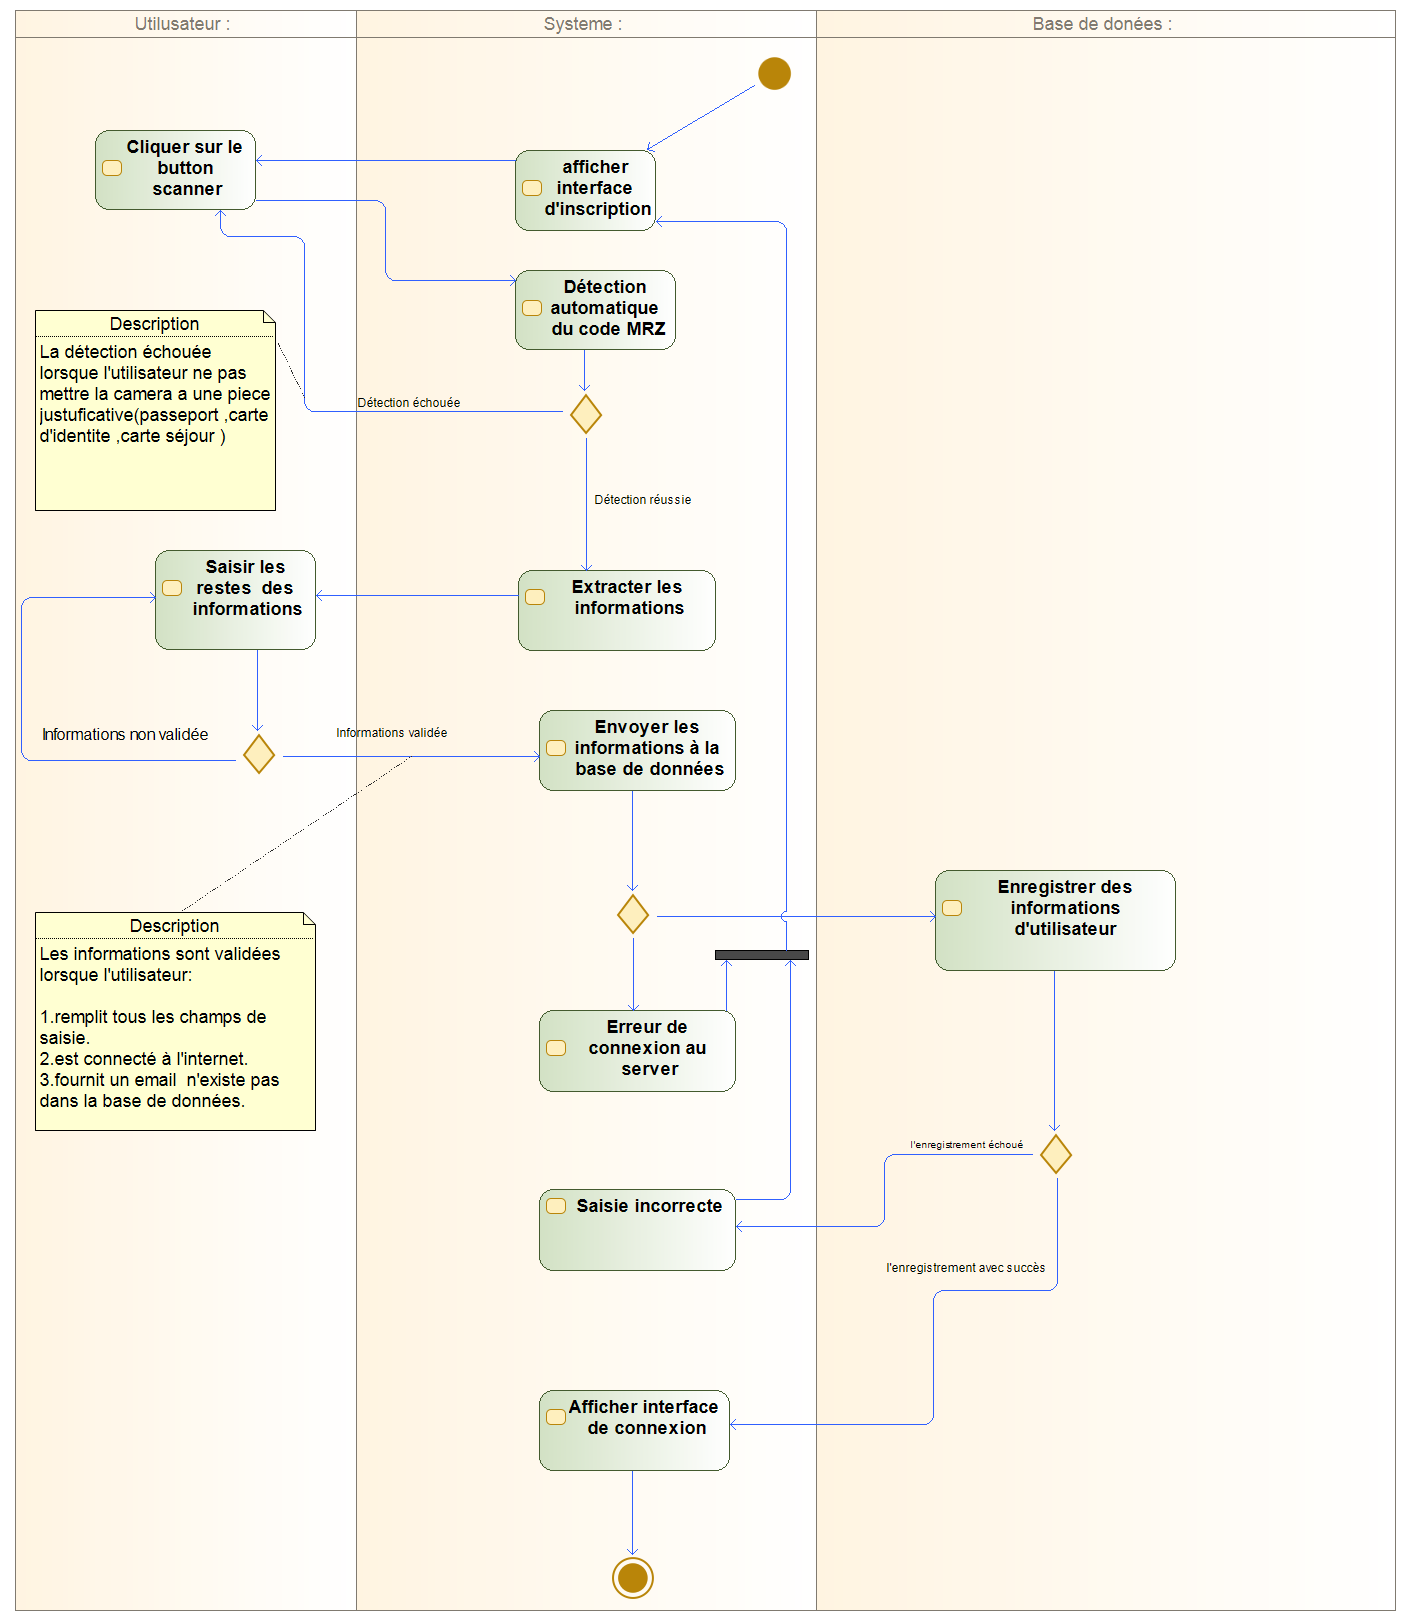
\includegraphics[width=18cm, height=19cm]{./Template LaTeX/Images/ins_act.png}
\caption{Diagramme d’activité : Création de compte}
\label{activiteCompte}

\end{figure}

\subsubsection{Transfert d'argent}
Le diagramme d’activité qu’illustre la figure~\ref{activiteTr} décrit les différentes actions ou enchainements
effectués lors d’une opération de transfert d’argent.
\begin{figure}[h!]
	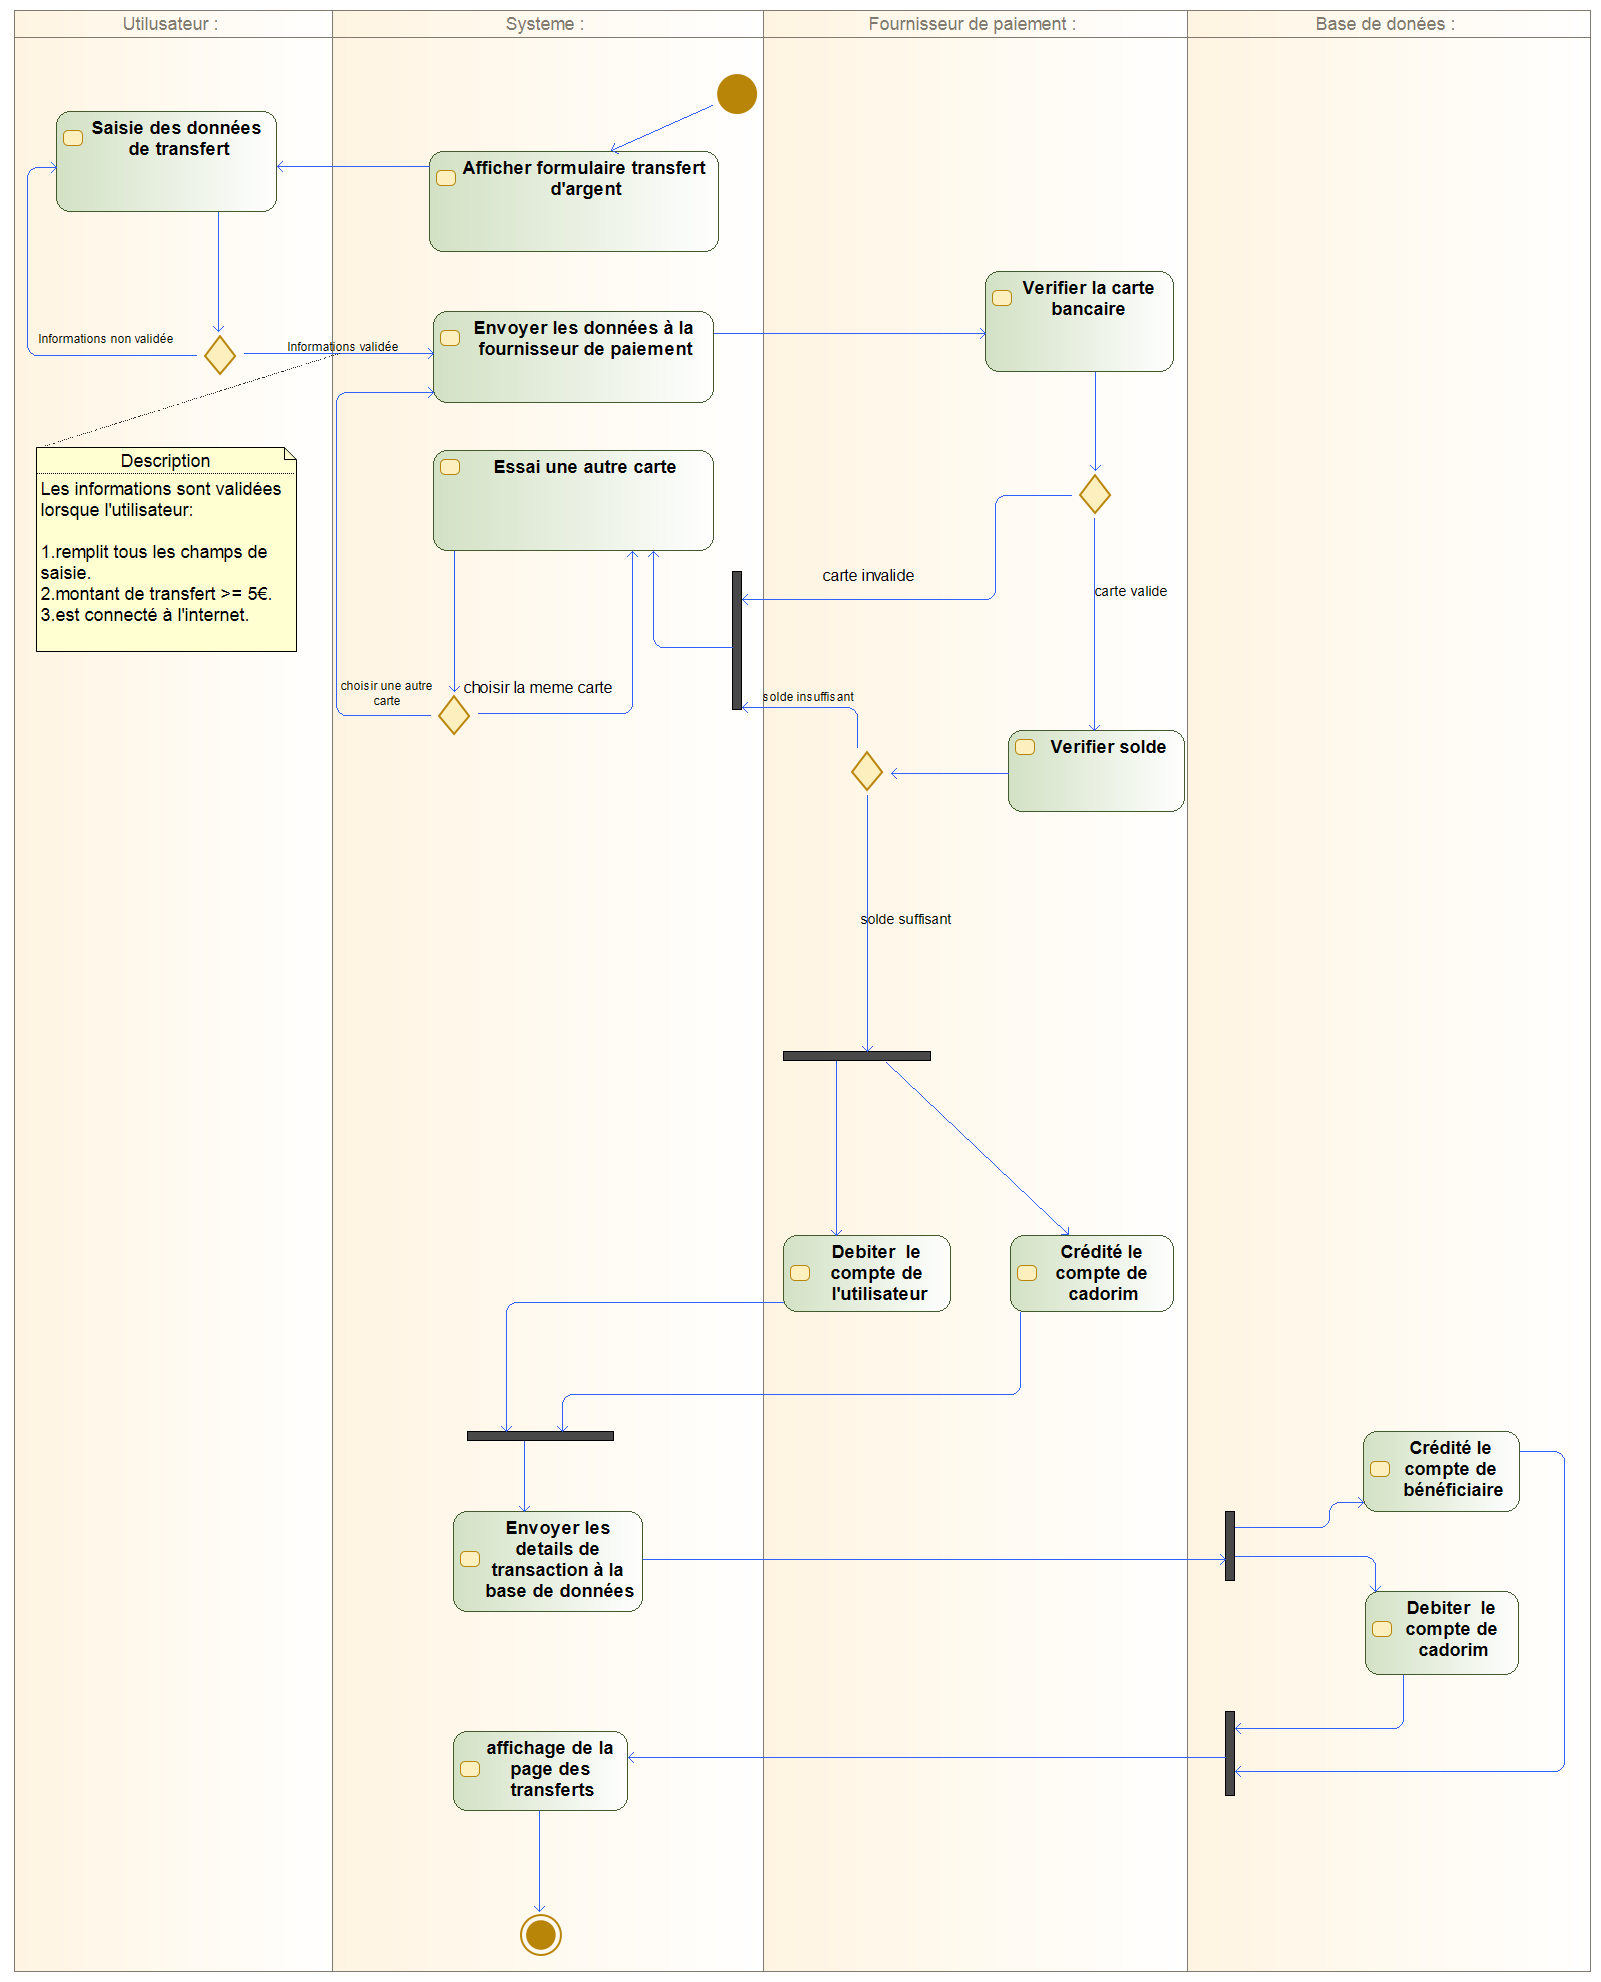
\includegraphics[width=18cm, height=20cm]{./Template LaTeX/Images/trans_act.png}
	\caption{Diagramme d'activité : Transfert d'argent}
	\label{activiteTr}
\end{figure}

\subsubsection{Authentification}
Le diagramme d’activité qu’illustre la figure~\ref{activiteAuth} décrit le cas d’utilisation « Authentification ».
\begin{figure}[h!]
	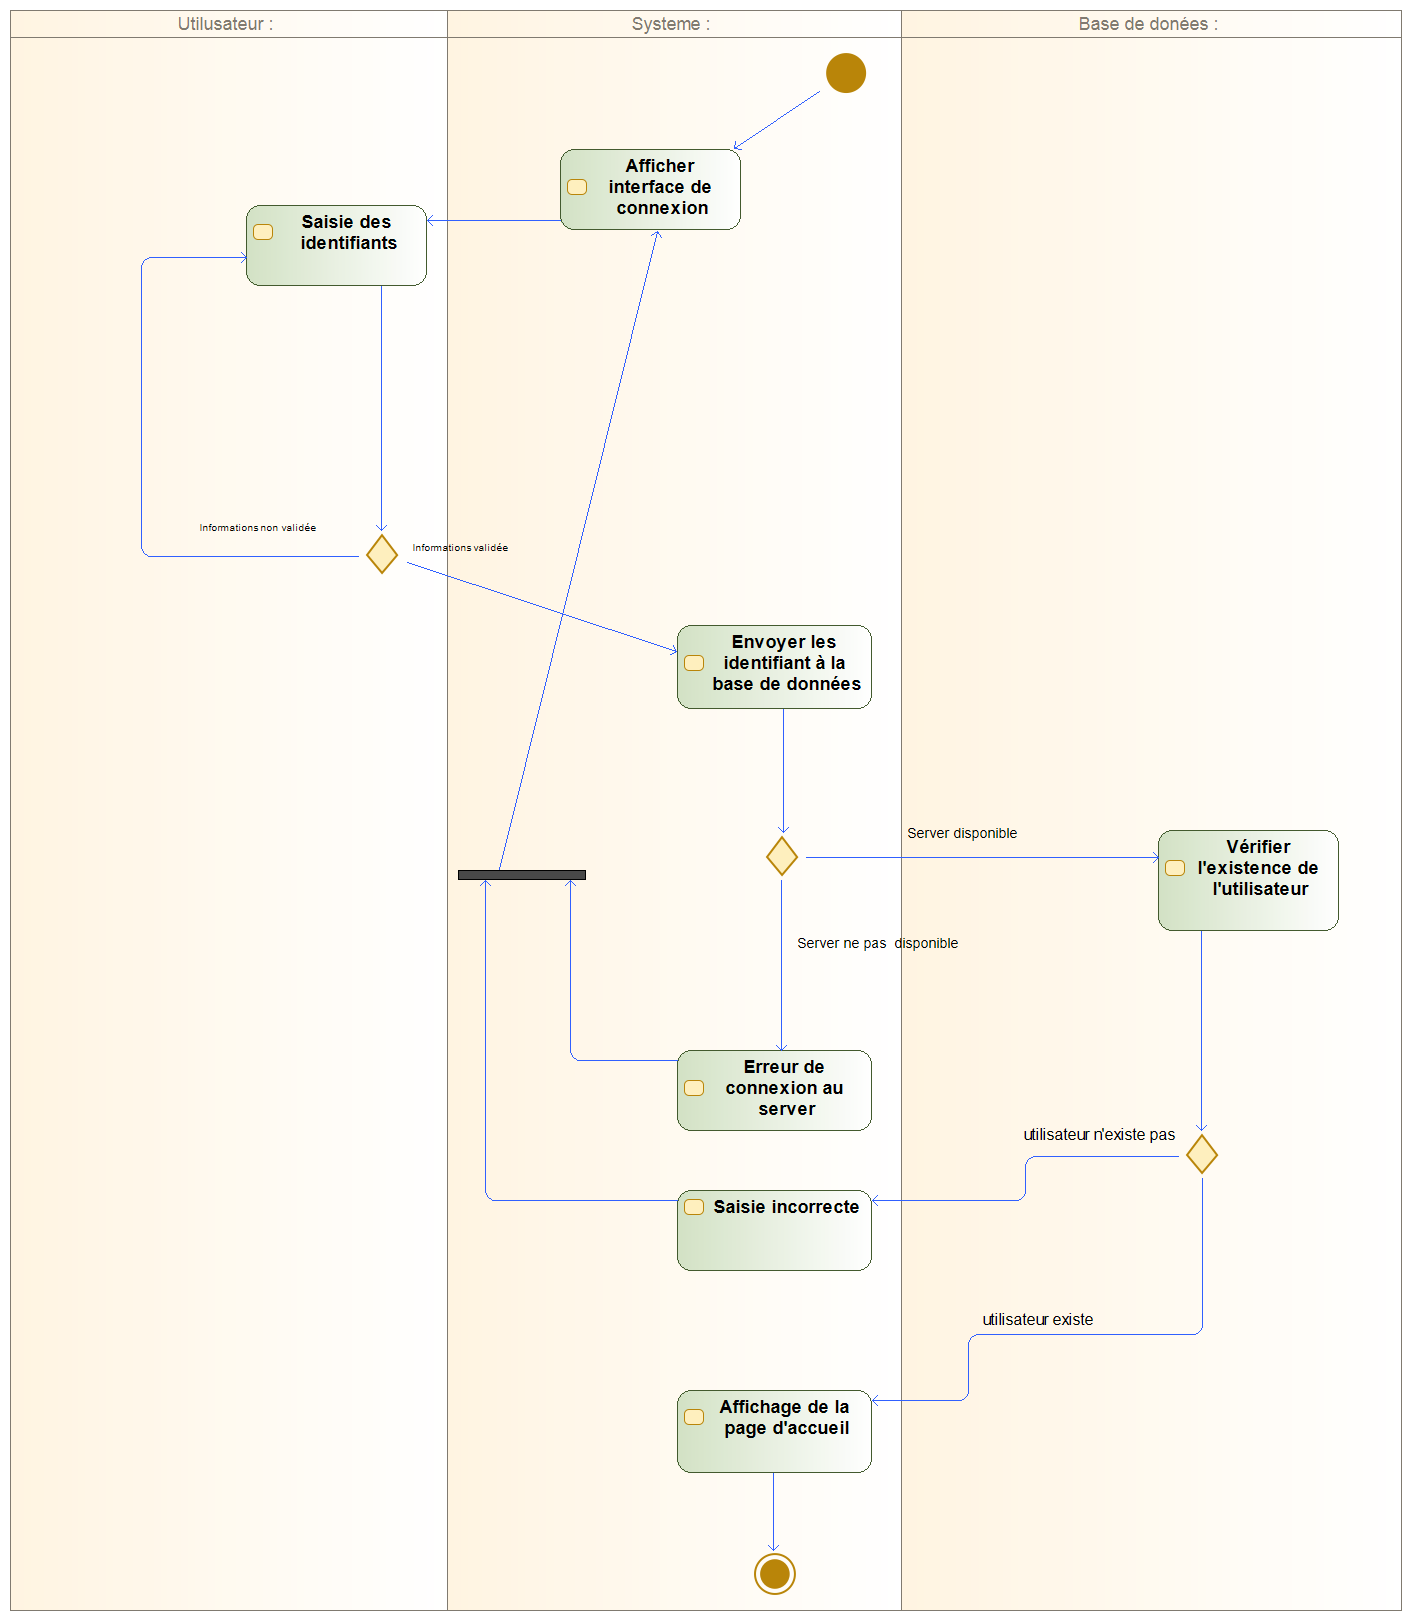
\includegraphics[width=18cm, height=20cm]{./Template LaTeX/Images/auth_act.png}
	\caption{Diagramme d'activité : Authentification}
	\label{activiteAuth}
\end{figure}


%\section{Modélisation de la base de données}
%\subsection{Diagramme de séquence}
%\newpage

\subsection{Diagramme de classe}
Afin de bien détailler l’architecture de la base de données, nous avons conçu le diagramme de
classe représenté dans la figure~\ref{fig4:class}.
\begin{figure}[h!]
	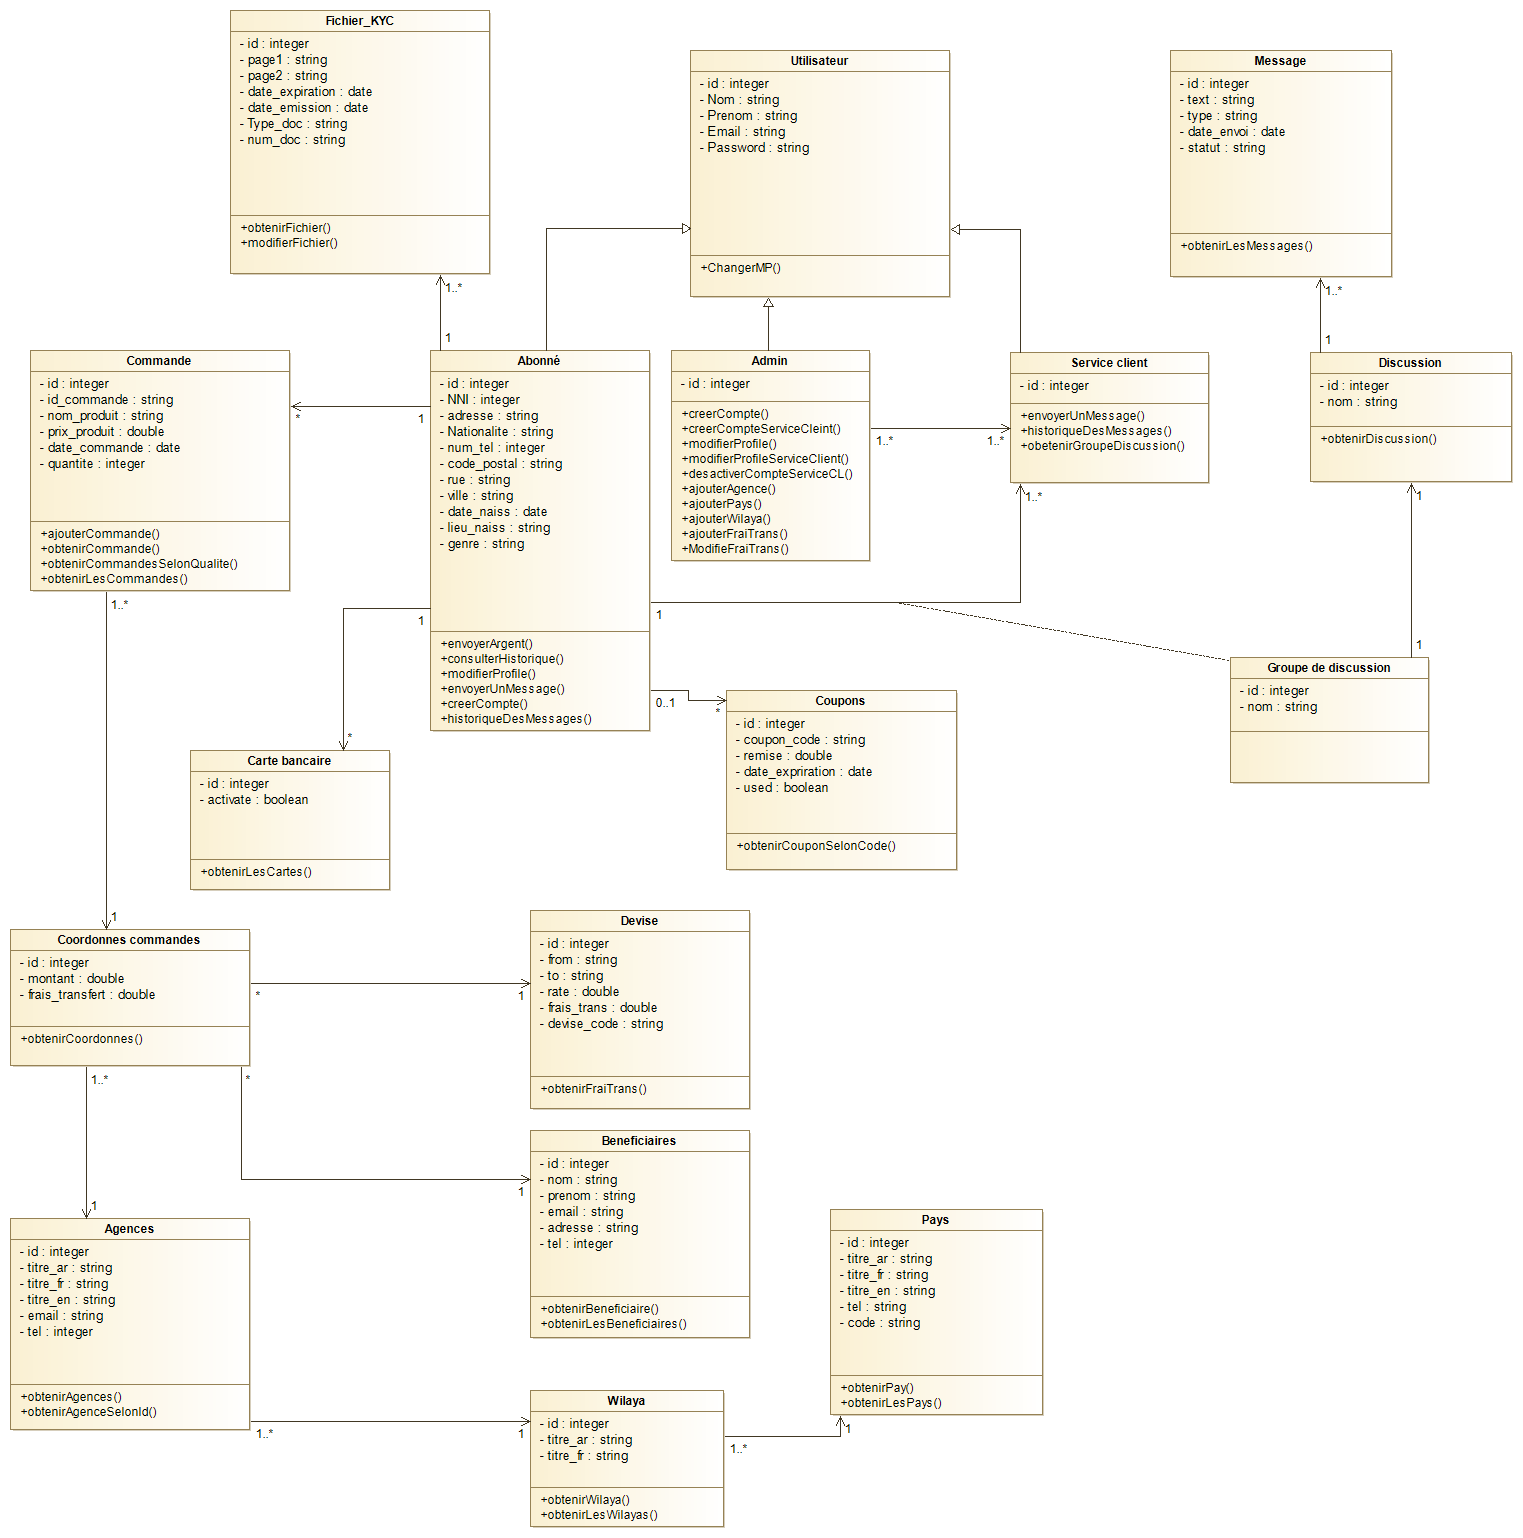
\includegraphics[width=18cm, height=20cm]{./Template LaTeX/Images/Diagramme_de_classe_V3.png}
	\caption{Diagramme de classe}
	\label{fig4:class}
\end{figure}
\newpage
\hspace*{-2cm} Le tableau~\ref{fig4:classT} explique les différentes classes de la base de données.
\begin{table}[h]
	\hspace*{-2cm}
	%\vspace*{6cm}
	\begin{tabular}{|m{5cm}|m{14cm}|}
		\hline
			\textbf{Classe}& \textbf{Description}
		\\
		\hline
		Abonné&Informations de l'utilisateur
		\\
		\hline
		Fichier KYC&  Contient les informations du fichier (carte d'identité, passeport, titre de séjour, carte bancaire) de client
		\\
			\hline
		Commande& Informations concernant une commande
		\\
			\hline
		Coordonnes commandes& Détails de chaque commande
		\\
			\hline
		Agences& Informations sur les agences de cadorim
		\\
			\hline
		Carte bancaire& Gestion de carte bancaire\\
		\hline	
			Devise& Informations sur la devise selon le pays d'envoi et le pays reçoivent
		\\
		\hline
			Beneficiaires&Informations sur les Beneficiaires
		\\
		\hline	
			Wilaya&Informations sur les Wilayas
		\\
		\hline	
			Admin&Informations de l’Admin et ses privilèges
		\\
		\hline	
			Service client&Service client avec certains privilèges
		\\
		\hline	
			Coupons&Informations d’un coupon
		\\
		\hline	
			Groupe de discussion&Informations sur les groupes
		\\
		\hline	
			Discussion&Informations de discussion de chaque groupe
		\\
		\hline		
			Message&Contient les messages de chaque discussion
		\\
		\hline
			Pays&Informations sur les pays
		\\
		\hline		
	\end{tabular}
	%\vspace*{10cm}
	\centering \caption{Description de la base de données}
	\label{fig4:classT}
\end{table}

%%%%%%%%%%%%%%%%%%%%%%%%%%%%%%%%%%%%%%%%%%%%5 ICI %%%%%%%%%%%%%%%%%%%%%%%%%%%%%%%%%%%%%%%%555


	
	
\end{document}